\documentclass{article}

% if you need to pass options to natbib, use, e.g.:
    \PassOptionsToPackage{numbers, compress}{natbib}
% before loading neurips_2026

% The authors should use one of these tracks.
% Before accepting by the NeurIPS conference, select one of the options below.
% 0. "default" for submission
\usepackage{neurips_2026}
% the "default" option is equal to the "main" option, which is used for the Main Track with double-blind reviewing.
% 1. "main" option is used for the Main Track
 % \usepackage[main]{neurips_2026}
% 2. "position" option is used for the Position Paper Track
%  \usepackage[position]{neurips_2026}
% 3. "eandd" option is used for the Evaluations & Datasets Track
 % \usepackage[eandd]{neurips_2026}
 % if you need to opt-in for a single-blind submission in the E&D track:
 %\usepackage[eandd, nonanonymous]{neurips_2026}
% 4. "creativeai" option is used for the Creative AI Track
%  \usepackage[creativeai]{neurips_2026}
% 5. "sglblindworkshop" option is used for the Workshop with single-blind reviewing
 % \usepackage[sglblindworkshop]{neurips_2026}
% 6. "dblblindworkshop" option is used for the Workshop with double-blind reviewing
%  \usepackage[dblblindworkshop]{neurips_2026}

% After being accepted, the authors should add "final" behind the track to compile a camera-ready version.
% 1. Main Track
 % \usepackage[main, final]{neurips_2026}
% 2. Position Paper Track
%  \usepackage[position, final]{neurips_2026}
% 3. Evaluations & Datasets Track
 % \usepackage[eandd, final]{neurips_2026}
% 4. Creative AI Track
%  \usepackage[creativeai, final]{neurips_2026}
% 5. Workshop with single-blind reviewing
%  \usepackage[sglblindworkshop, final]{neurips_2026}
% 6. Workshop with double-blind reviewing
%  \usepackage[dblblindworkshop, final]{neurips_2026}
% Note. For the workshop paper template, both \title{} and \workshoptitle{} are required, with the former indicating the paper title shown in the title and the latter indicating the workshop title displayed in the footnote.
% For workshops (5., 6.), the authors should add the name of the workshop, "\workshoptitle" command is used to set the workshop title.
% \workshoptitle{WORKSHOP TITLE}

% "preprint" option is used for arXiv or other preprint submissions
 % \usepackage[preprint]{neurips_2026}

% to avoid loading the natbib package, add option nonatbib:
%    \usepackage[nonatbib]{neurips_2026}

\usepackage[utf8]{inputenc} % allow utf-8 input
\usepackage[T1]{fontenc}    % use 8-bit T1 fonts
\usepackage{hyperref}       % hyperlinks
\usepackage{url}            % simple URL typesetting
\usepackage{booktabs}       % professional-quality tables
\usepackage{amsfonts}       % blackboard math symbols
\usepackage{nicefrac}       % compact symbols for 1/2, etc.
\usepackage{microtype}      % microtypography
\usepackage[dvipsnames]{xcolor}         % colors
\usepackage{amsmath}
\usepackage{graphicx}
\usepackage{csquotes}
\usepackage{amsthm}
\usepackage{wrapfig}
\usepackage{subcaption}
\usepackage{dirtytalk}
\usepackage{multirow}
\usepackage{mathtools}
\usepackage{array}
\usepackage{amsmath}
\usepackage{amsthm}
\usepackage[inline]{enumitem}
\usepackage{tabularray}
\usepackage[most]{tcolorbox}
\definecolor{bg_yellow}{HTML}{FCFCE3}
\definecolor{title_yellow}{HTML}{F4EEAC}

\newtcolorbox{road2}{
  colback=bg_yellow,
  enhanced,
  title=,
  attach boxed title to top left,
  fonttitle=\bfseries,
  coltitle=black,
  toprule=0pt,
  bottomrule=0pt,
  rightrule=0pt,
  leftrule=3pt,
  arc=0mm,
  skin=enhancedlast jigsaw,
  sharp corners,
  colframe=bg_yellow,
  colbacktitle=title_yellow,
  boxed title style={
    frame code={
      \fill[title_yellow] 
        (frame.south west) -- 
        (frame.north west) -- 
        (frame.north east) -- 
        ([xshift=3mm]frame.east) -- 
        (frame.south east) -- 
        cycle;

      \draw[line width=1mm, title_yellow] 
        ([xshift=2mm]frame.north east) -- 
        ([xshift=5mm]frame.east) -- 
        ([xshift=2mm]frame.south east);

      \draw[line width=1mm, title_yellow] 
        ([xshift=5mm]frame.north east) -- 
        ([xshift=8mm]frame.east) -- 
        ([xshift=5mm]frame.south east);

    }
  }
}


\UseTblrLibrary{booktabs}
\theoremstyle{definition}
\newtheorem{definition}{Definition}[section]
\newtheorem{notation}{Notation}[section]
\newtheorem{example}{Example}[section]

\theoremstyle{remark}
\newtheorem*{remark}{Remark}

\newtheorem{proposition}{Proposition}[section]
\newtheorem{theorem}{Theorem}[section]

% Note. For the workshop paper template, both \title{} and \workshoptitle{} are required, with the former indicating the paper title shown in the title and the latter indicating the workshop title displayed in the footnote. 
\title{Explicit and Effectively Symmetric Schemes for Neural SDEs}


% The \author macro works with any number of authors. There are two commands
% used to separate the names and addresses of multiple authors: \And and \AND.
%
% Using \And between authors leaves it to LaTeX to determine where to break the
% lines. Using \AND forces a line break at that point. So, if LaTeX puts 3 of 4
% authors names on the first line, and the last on the second line, try using
% \AND instead of \And before the third author name.

\author{%
  Daniil Shmelev\\
  Department of Mathematics\\
  Imperial College London\\
  \texttt{daniil.shmelev23@imperial.ac.uk} \\
  \And
  Maybe me?\\
  we should discuss\\
  \And
  Cristopher Salvi\\
  Department of Mathematics\\
  Imperial College London\\
  \texttt{c.salvi@imperial.ac.uk} \\
}


\begin{document}


\maketitle


\begin{abstract}
  The abstract paragraph should be indented \nicefrac{1}{2}~inch (3~picas) on both the left- and right-hand margins. Use 10~point type, with a vertical spacing (leading) of 11~points. The word \textbf{Abstract} must be centered, bold, and in point size 12. Two line spaces precede the abstract. The abstract must be limited to one paragraph.
\end{abstract}


\newcommand{\luke}[1]{\textcolor{blue}{#1}}
\luke{I have shortened the below by a few lines (mostly the blockquote) as space is needed for extra experiments. we probably should hint more at optimal memory}
\section{Introduction}
\emph{Neural stochastic differential equations (SDEs)} have emerged as a flexible tool for modeling stochastic dynamics, with training typically cast as a distribution-matching problem between generated and observed trajectories. Several approaches have been proposed in the literature, differing mainly in the choice of discriminating divergence. SDE-GANs~\citep{kidger2021neural} use the 1-Wasserstein distance, while Latent SDEs~\citep{li2020scalable} optimize with respect to the KL divergence via variational inference, and can be viewed as variational autoencoders. Another alternative proposed by~\cite{issa2023non} trains neural SDEs non-adversarially using maximum mean discrepancies (MMD) with \emph{signature kernels}~\citep{kiraly2019kernels, salvi2021signature, lemercier2024log}, a recently introduced family of kernels on path space which received significant attention due to their efficiency in handling path-dependent problems~\citep{salvi2021higher, lemercier2021distribution, pannier2024path, cirone2025rough}.

While effective, the stochastic calculus underpinning SDEs can be technically cumbersome, especially when developing higher order solvers, deriving and analyzing backpropagation algorithms, or extending to rougher noises than Brownian motion. A natural way to bypass these limitations is to view SDEs through the lens of \emph{rough paths}. Rough path theory \citep{lyons1998differential, gubinelli2004controlling, gubinelli2010ramification} provides a deterministic calculus on path space that extends classical It\^o integration beyond semimartingales, enabling one to treat SDEs as a special case of \emph{rough differential equations (RDEs)}
\begin{equation}\label{eqn:rde}
\mathrm{d}y(t) \;=\; f_0(t, y_t)\,\mathrm{d}t \;+\; f(t, y_t)\,\mathrm{d}\mathbf{X}(t), 
\qquad y_{t_0} = y_0 \in \mathbb{R}^m, \tag{RDE}
\end{equation}
where $\mathbf{X}$ is a \emph{rough path} above a driving signal $X = (X^1,...,X^d) : [0,T] \to \mathbb{R}^d$, $f = (f_1,...,f_d)$ and $f_i : \mathbb{R}^m \to \mathbb{R}^m$ are  vector fields for $i=0,...,d$ which determine the system dynamics. In fact, there is a large class of stochastic processes which can be “naturally lifted” to rough paths, including Gaussian processes such as fractional Brownian motion with Hurst parameter $H > 1/4$ and Volterra processes \citep{friz2010multidimensional}. Viewing SDEs through the lens of RDEs yields a significant conceptual simplification. In the RDE framework, the driving signal $\mathbf{X}$ is treated as a rough path, abstracting away the stochastic integral and allowing one to work with deterministic calculus on path space. Rough path theory has become a powerful framework for analyzing modern machine learning models. It has provided the foundation for proving theoretical properties of neural differential equations~\citep{morrill2021neural, arribas2020sigsdes, cirone2023neural, holberg2024exact}, sequence-to-sequence architectures~\citep{kidger2019deep}, and, more recently, deep selective state-space models (SSMs)~\citep{cirone2024theoretical, cirone2025parallelflow, walker2025structured} and score-based diffusion models~\citep{barancikovasigdiffusions}. For a survey of recent applications of rough path theory to machine learning, we refer the reader to~\citep{fermanian2023new}.

From an algorithmic perspective, the RDE formulation also plays a central role in training neural SDEs (NSDEs), where one must backpropagate through an SDE solver. In particular, the derivation of the \emph{adjoint method}---a key tool for differentiation through differential equation solvers---is considerably more transparent in the RDE setting, avoiding much of the technical machinery required in the stochastic case; see, for instance,~\citep[Sec.~3.3.4]{cass_salvi_notes}. More broadly, the RDE viewpoint unifies backpropagation across ODEs, SDEs, and controlled differential equations (CDEs)~\citep{kidger2020neural}, providing a clean pathwise calculus that is both mathematically rigorous and naturally aligned with autodiff frameworks. Several strategies have been proposed. A first, often called \emph{discretise-then-optimise}, differentiates directly through the solver’s internal operations. This yields accurate gradients and is computationally efficient, but requires storing all intermediate states and is therefore memory-intensive. A second, \emph{optimise-then-discretise}, instead derives a backward-in-time adjoint equation and solves it numerically via a second call to the solver. This removes the need to store intermediate quantities, giving constant memory cost with respect to solver depth. However, it typically produces less accurate gradients and is slower, since the forward trajectory must be recomputed during the backward pass.

A third option leverages \emph{algebraically reversible solvers}, which enable exact reconstruction of the solution trajectory from the terminal state, and hence permit accurate and memory-efficient backpropagation. In the setting of an autonomous ODE
\begin{equation} \label{eq:ode}
    \mathrm{d}y_t = f(y_t) \, \mathrm{d}t,
\end{equation}
a one-step method $y_{n+1} = y_n + \Phi_h(y_n)$ is \emph{reversible} or \emph{symmetric} if a step of the method starting from $y_1$ with negative step size exactly recovers the initial condition $y_0$, that is, $\Phi_{-h} = \Phi_h^{-1}$. Although reversible schemes are appealing for backpropagation through differential equations, they are difficult to construct. Classical Runge--Kutta schemes are reversible only if they are implicit \citep[Sec.~2.1]{hairer2006geometric}, making them unsuitable for applications to Neural ODEs. More generally, symmetric parasitism-free\footnote{Here, \emph{parasitism} refers to spurious numerical modes of a general linear method, arising from non-principal eigenvalues and not from the true ODE dynamics, which may contaminate the computed solution.} general linear methods cannot be explicit \citep{butcher2016symmetric}. To avoid implicitness, existing reversible methods such as the asynchronous leapfrog integrator (ALF) \citep{zhuang2021mali} and Reversible Heun \citep{kidger2021efficient} instead track auxiliary states during integration. This yields explicit reversible schemes, but enlarges the effective state dimension and thereby reduces their practical memory advantage. These methods can also be unstable in practice on more challenging problems. For example, \citet{zhang2021path} report:

\begin{displayquote}
\textit{``...[W]e found [Reversible Heun] is less stable compared with simple Euler integration without adjoint and results in numerical issues occasionally. ... methods without adjoint are more stable and lower loss compared with adjoint ones...''~\citep{zhang2021path}}
\end{displayquote}

A potential solution to the difficulties of reversible solvers comes with the class of \emph{Explicit and Effectively Symmetric (EES)} Runge--Kutta schemes introduced in \cite{shmelev2025explicit}. Instead of considering exactly reversible schemes, the authors propose schemes which are almost reversible, up to an acceptable tolerance level. Such schemes offer stable, explicit integration methods which are virtually indistinguishable from truly symmetric schemes in practice. The authors demonstrate the efficacy of EES schemes on classical ODEs, and show that EES schemes are capable of producing similar results to classical schemes such as RK3 and RK4. In \cite{shmelev2025explicit}, the formulation of EES schemes is limited to ODEs, without an explicit generalisation to the case of SDEs or RDEs. \luke{Our development shows that this framework extends beyond Euclidean ODEs, and can be realised in forms that are better suited to training: low-storage implementations, adaptive error control, and manifold-valued integration.}

Derivative-free \emph{Runge--Kutta (RK) methods} for RDEs were introduced by \cite{redmann2022runge}. Similarly to classical RK schemes for ODEs, the study of these methods is conducted through the formalism of B-series ~\citep{hairer2006geometric,mclachlan2015butcher,butcher2021b}. A B-series is an infinite series representation of a method, indexed by (labelled) non-planar rooted trees. A brief overview of B-series is given in Appendix \ref{appendix:trees}. A natural consequence of this analysis is that a general Runge--Kutta method for RDEs is given in terms of tree-iterated integrals of the underlying driving process. In practice, these tree-iterated integrals cannot be simulated directly as their distributions are often intractable. Following~\citep{deya2012milstein}, \cite{redmann2022runge} replaced these tree-iterated integrals with products of increments of the driving path. This substitution simplifies the derivation of Runge--Kutta coefficients and makes it feasible to establish order conditions up to any desired order.
\clearpage
\luke{In this paper, we formulate EES Runge--Kutta schemes for RDEs, develop practical low-storage and adaptive variants, and show that the same construction extends naturally to manifold-valued settings. We demonstrate their effectiveness for Neural SDE training.} Our main contributions are as follows:
\begin{enumerate}[]
    \item We extend EES Runge--Kutta schemes to the RDE setting, yielding explicit effectively symmetric integrators applicable to Neural SDEs.
    \item We introduce new EES schemes, including a $2N$ low-memory schemes and FSAL methods with embedded error estimates to yield memory-efficient and error-adaptive solvers.
    \item We show that this low-storage EES construction extends cleanly to homogeneous manifold integrators, yielding efficient methods for Riemannian diffusion models.
    \item We establish their theoretical and empirical advantages for Neural SDE training, including improved stability over existing reversible solvers and lower gradient errors.
    \item We release open-source implementations of the standard, low-memory, and manifold EES schemes in PyTorch, JAX, and Julia, facilitating adoption by the research community.
\end{enumerate}
The remainder of the paper is organized as follows. Section \ref{sec:rev_solvers} reviews reversible methods for neural differential equations, memory-efficient schemes, and their relation to manifold methods. Section \ref{sec:ees} introduces EES schemes for ODEs, extends them to RDEs, and develops their low-storage, adaptive, and manifold-valued variants, together with convergence, stability, and backpropagation results. Section \ref{sec:experiments} evaluates the proposed methods on synthetic and real-world Neural SDE benchmarks. Section \ref{sec:conclusion} concludes with limitations and future directions.

\section{Preliminaries}
\luke{The idea of this preliminaries is to better separate our contributions from those we take from the literature}
\subsection{Existing Reversible ODE and SDE Solvers}
\luke{not quite clear which reversible solvers were just given for ODE vs which are for SDE. may confused reviewers}
A limited number of efficient reversible solvers have been proposed in the literature. The asynchronous leapfrog integrator (ALF) ~\citep{zhuang2021mali} for Neural ODEs overcomes the barrier of implicit schemes by tracking an additional state $v$ as part of the integration. Applied to the ODE \eqref{eq:ode}, the update rule of the ALF scheme can be written as
\begin{align*}
    y_{n+2} &= y_n + h f\left(t_n + \frac{h}{2}, y_n + \frac{h}{2} v_n\right),\\
    v_{n+2} &=2f\left(t_n + \frac{h}{2}, y_n + \frac{h}{2} v_n\right) - v_n.
\end{align*}
For SDEs of the form $dy_t = g(t,y_t)dt + f(t,y_t)dW_t$, the Reversible Heun method ~\citep{kidger2021efficient} takes a similar approach, reading
\begin{align*}
    y_{n+1} &= y_n + \frac{1}{2}(g(t_n, v_n) + g(t_{n+1}, v_{n+1})) \Delta t + \frac{1}{2}(f(t_n, v_n) + f(t_{n+1}, v_{n+1})) \Delta W_n,\\
    v_{n+1} &= 2y_n - v_n + g(t_n, v_n) \Delta t + f(t_n, v_n) \Delta W_n.
\end{align*}
The Reversible Heun method is efficient, requiring only one evaluation of the drift $g$ and the diffusion $f$ per step. However, the method is known to be inherently unstable \cite[Theorem D.19]{kidger2021efficient}.

To ameliorate this instability, \citet{mccallum2024efficient} propose a method transforming any ODE integration scheme $y_{n+1} = y_n + \Psi_h(t,y_n)$ into one which is reversible and with often larger stability domain than ALF and reversible Heun. They take the update
\begin{align*}
    y_{n+1} &= \lambda y_n + (1-\lambda) v_n + \Psi_h(t,v_n),\\
    v_{n+1} &= v_n - \Psi_{-h}(t_{n+1}, y_{n+1}),
\end{align*}
for a given coupling parameter $\lambda \in (0,1]$. Nonetheless, the resulting stability domain remains much smaller than the that of the underlying method $\Psi$, and additionally on the coupling parameter $\lambda$.

\luke{In all cases, these methods break the strict RK structure, so they do not necessarily admit clean manifold generalizations as stnadard RK schemes do via RKMK. Furthermore, they must expand the state space, making them non memory optimal and so on}

\subsection{EES Schemes for ODEs}

EES schemes~\citep{shmelev2025explicit} are a class of explicit Runge--Kutta methods which offer an efficient approach to reversible integration without compromising stability, while retaining the standard explicit Runge--Kutta form. Given positive integers $m \geq n$, an explicit Runge--Kutta scheme $\Phi_h$ is said to be an $\mathrm{EES}(n,m)$ scheme if $\Phi_h$ is of order $n$ and $\Phi_{-h} \circ \Phi_h$ recovers the initial condition up to order $m$ when applied to an ODE. When $m$ is large, such schemes exhibit near-reversible behaviour, which is often sufficient in practice. In~\cite{shmelev2025explicit}, Butcher tableaux are derived for 3-stage $\mathrm{EES}(2,5)$ and 4-stage $\mathrm{EES}(2,7)$ schemes. Although the emphasis there is mostly on $\mathrm{EES}(2,7)$, for our Neural SDE applications we restrict attention to $\mathrm{EES}(2,5)$, since we do not expect the additional accuracy of $\mathrm{EES}(2,7)$ to justify the extra stage in our setting. Proposition~\ref{prop:EES_2_5} gives the general one-parameter family of $\mathrm{EES}(2,5)$ tableaux, which we denote by $\mathrm{EES}(2,5;x)$.
\begin{proposition}[{\cite[Proposition 8.4]{shmelev2025explicit}}]
\label{prop:EES_2_5}
    For $x \in \mathbb{R} \setminus \{1,\pm \frac{1}{2}\}$, 3-stage Runge--Kutta schemes belonging to $\mathrm{EES}(2,5)$ have Butcher tableau
    \begin{equation}
    {\renewcommand{\arraystretch}{2.2}
    \begin{array}{c|ccc}
    0 &&&\\
    \displaystyle\frac{1+2x}{4(1-x)} & \displaystyle\frac{1+2x}{4(1-x)} &&\\[7pt]
    \displaystyle\frac{3}{4(1-x)} & \displaystyle\frac{(4x-1)^2}{4(x-1)(1-4x^2)} & \displaystyle\frac{1-x}{(1-4x^2)} &\\[7pt]
    \hline
    & x & \displaystyle\frac{1}{2} & \displaystyle\frac{1}{2} - x
    \end{array}
    }
    \end{equation}
\end{proposition}

\begin{wrapfigure}{r}{5cm}
\vspace{-3em}
    
\includegraphics[width = 0.4\textwidth]{figures/stability_regions_1.pdf}
    \captionsetup{oneside,margin={0.5cm,0cm}}
    \caption{\textit{Stability domain for $\mathrm{EES}(2,5;1/10)$ compared to Kutta's RK3 and RK4.}}
    \label{fig:ees25_stability}
    \vspace{-2em}
\end{wrapfigure}

The stability region for $\mathrm{EES}(2,5)$ is comparable to classical methods such as Kutta's RK4, significantly larger than those of ALF and Reversible Heun whose region is the line $[-i,i]$. Theorem~\ref{thm:ees25_ode_stability} gives the exact form of this region for $\mathrm{EES}(2,5;x)$.

\begin{theorem}\label{thm:ees25_ode_stability}
    Suppose that, for some $x \neq 1, \pm \frac{1}{2}$, $\mathrm{EES}(2,5;x)$ is used to obtain a solution $\{y_n\}_{n \geq 0}$ to the linear test equation $dy = \lambda y\, dt$, where $\lambda \in \mathbb{C}$ and $y_0 \neq 0$. Then $y_n \to 0$ as $n \to \infty$ if and only if
    \begin{equation*}
        \left\lvert 1 + \rho + \frac{1}{2} \rho^2 + \frac{1}{8} \rho^3 \right\rvert < 1, \qquad \rho = \lambda h.
    \end{equation*}
\end{theorem}

This follows by a direct computation of the stability function
$R(\rho)=1+\rho+\frac{1}{2}\rho^2+\frac{1}{8}\rho^3$,
which is independent of $x$. Following \citet[Section 8.1]{shmelev2025explicit}, we fix $1/10$ and refer to $\mathrm{EES}(2,5;1/10)$ as \textit{the} $\mathrm{EES}(2,5)$ scheme. \luke{we should plot rev Heun and ALF as a line from -i,i somehow.} 

Beyond stability and near-reversibility, EES(2,5) has an additional structural property we exploit in the sequel, namely, that it permits realization as a $2N$ scheme.

%%%%%%%%%%%%%%%%%%%%%%%%%%%%%%%%%%%%%%%%%%%%%%%%%%%%%%%%%%%%
\section{Explicit and Effectively Symmetric (EES) schemes for RDEs}\label{sec:ees}
\subsection{A $2N$ realization of $\mathrm{EES}(2,5)$}

The key structural observation used in our construction is that the chosen
$\mathrm{EES}(2,5)$ scheme is a Williamson-type $2N$ Runge--Kutta method. Recall that a $2N$ method admits a recurrence of the form
\begin{equation}
\label{eq:2n_rk}
\begin{aligned}
    \Delta Y_i &= A_i \Delta Y_{i-1} + h\, f(Y_{i-1}), \\
    Y_i &= Y_{i-1} + B_i \Delta Y_i,
\end{aligned}
\qquad i=1,\dots,s.
\end{equation}
Thus, for a state of size $N$, an $s$-stage implementation requires only $2N$
registers, compared with $(s+1)N$ for a standard explicit Runge--Kutta method.

From the tableau \ref{prop:EES_2_5} it is clear that $\mathrm{EES}(2,5;x)$ admits such a low memory representation. Using the above memory complexities, this formulation \textbf{halves the memory requirement} of $\mathrm{EES}(2,5;x)$ from $4N$ to $2N$. We formalize this with the following proposition. The two-register recurrence structure also enables lifting to a homogeneous manifold integrator, which we utilize in Section~\ref{subsec:experiment_manifold_sde}.

\begin{theorem}[{\cite[Theorem~2]{bazavov_2n-storage_2025}}]
\label{thm:2N_relationship}
An explicit Runge--Kutta method is a Williamson $2N$ method iff
\[
a_{ij}(b_{j-1}-a_{j,j-1})=(a_{i,j-1}-a_{j,j-1})b_j,
\qquad i=3,\dots,s,\quad j=2,\dots,i-1.
\]
\end{theorem}

\begin{proposition}
\label{thm:all-ees25-are-2n}
For every admissible parameter $x \in \mathbb{R}\setminus\{1,\pm \frac12\}$,
the method $\mathrm{EES}(2,5;x)$ is a Williamson $2N$ scheme.
\end{proposition}

The proof in Appendix~\ref{prf:all-ees25-are-2n} proceeds by substituting the 
coefficients of Proposition~\ref{prop:EES_2_5} into the criterion of 
Theorem~\ref{thm:2N_relationship}; since $\mathrm{EES}(2,5;x)$ is 3-stage, 
only one identity requires verification, which holds for all admissible $x$. 
The recurrence \eqref{eq:2n_rk} serves as the starting point for the manifold 
construction in Section~\ref{subsec:experiment_manifold_sde}. In the context 
of neural ODEs and SDEs, the $2N$ formulation is particularly advantageous: 
standard discretize-then-optimize schemes must retain all intermediate solver 
states for backpropagation, whereas reversibility permits recomputation of 
forward states during the backward pass, ensuring that only $2N$ registers 
are required at any point in time.

%%%%%%%%%%%%%%%%%%%%%%%%%%%%%%%%%%%%%%%%%%%%%%%%%%
\subsection{Simplified Runge--Kutta Methods for RDEs}
We consider rough differential equations (RDEs) of the form
\begin{equation}\label{eq:rde}
    dy_t = f(y_t)\, d\mathbf{X}_t,
\end{equation}
where $\mathbf{X}$ is an $\alpha$-H\"older branched rough path, $\alpha \in (0,1]$, 
and $f$ is smooth and bounded with bounded derivatives; see Appendix 
\ref{appendix:branched_rp} for background. Following \citet{redmann2022runge}, 
we assume $\mathbf{X}$ is geometric, i.e.\ there exist smooth approximations 
$\{X^h\}_{h>0}$ whose natural lifts $\{\mathbf{X}^h\}_{h>0}$ satisfy 
$\varrho_\alpha^g(\mathbf{X}^h, \mathbf{X}) = \mathcal{O}(h^{r_0})$ for some 
$r_0 > 0$, where $\varrho_\alpha^g$ is the inhomogeneous geometric rough path 
metric. For convergence rates of such approximations for Gaussian processes, 
see \cite{friz2014convergence}. Letting $y^h$ denote the solution to 
\eqref{eq:rde} driven by $\mathbf{X}^h$, a simplified Runge--Kutta scheme 
for $y^h$ on an equidistant grid with stepsize $h$ is given by
\begin{align}\label{eq:simple_rk}
    y^h_{n+1} &= y^h_n + \sum_{m=1}^d\sum_{i=1}^s b_i f_m(k_i) X^{(m)}_{t_n, t_{n+1}},\\
    k_i &= y^h_n + \sum_{m=1}^d\sum_{j=1}^s a_{ij} f_m(k_j) X^{(m)}_{t_n, t_{n+1}},\nonumber
\end{align}
where $X^{(m)}_{t_n,t_{n+1}}$ denotes the $m$-th component increment of $X^h$ 
over $[t_n, t_{n+1}]$. Convergence rates for schemes of the form 
\eqref{eq:simple_rk} from \citet{redmann2020runge} are recalled in Appendix 
\ref{appendix:convergence_simplified}.

\subsection{Stability of EES schemes for SDEs}
%%%%%%%%%%%%%%%%%%%%%%%%%%%%%%%%%%%%%%%%%%%%%%%%%%

As discussed in the introduction and subsequently in Section \ref{sec:ees}, $\mathrm{EES}$ schemes offer a stable alternative to reversible integration. Whilst the stability of $\mathrm{EES}$ in the case of ODEs has been studied in \citet{shmelev2025explicit} and Section \ref{sec:ees}, we are interested in the stability of $\mathrm{EES}_\mathcal{R}$ when applied to stochastic drivers for our applications to Neural SDEs. To evaluate the stability in the context of SDEs, we consider the \textit{mean-square stability}, which has been widely used for the analysis of stochastic integration methods in the literature ~\citep{higham2000mean, drummond1991computer, hernandez1993convergence, komori1995stahle, komori1994some, petersen1998general, saito1993t, saito1996stability, schurz1996asymptotical}. Given the test equations
\begin{equation}\label{eq:sde_test_eq}
    dy_t = \lambda y_t dt + \mu y_t dW_t,
\end{equation}
where $\lambda, \mu \in \mathbb{C}$ and $y_0 \neq 0$ almost surely, a solution $\{y_n\}_{n \geq 0}$ derived from a numerical integrator is said to be \textit{mean-square stable} if $\lim_{n \to \infty} \mathbb{E}(|y_n|^2) = 0$. It follows in a similar fashion to Theorem \ref{thm:ees25_ode_stability} that $\mathrm{EES}(2,5;x)$ applied to \ref{eq:sde_test_eq} is mean-square stable if and only if
\begin{equation*}
    \mathbb{E} \left[ \left\lvert 1 + \rho + \frac{1}{2} \rho^2 + \frac{1}{8} \rho^3 \right\rvert^2 \right] < 1,
\end{equation*}
where $\rho = \lambda dt + \mu dW_t \sim N(\lambda dt, \mu^2 dt)$. Figure 
\ref{fig:ees_stoch_stability} shows 4 cross-sections of the stability domain. 
For comparison, we take the RDE analogues of RK3 and RK4 in 
\eqref{eq:simple_rk}, $\mathcal{R}(\text{RK3})$ and $\mathcal{R}(\text{RK4})$. 
Along most cross-sections, $\mathrm{EES}_\mathcal{R}(2,5)$ achieves similar 
or greater stability than $\mathcal{R}(\text{RK3})$ and $\mathcal{R}(\text{RK4})$.

\begin{figure}[h]
\centering
    
\includegraphics[width = \textwidth,trim={0.95cm .3cm 0cm .4cm},clip]{figures/stoch_stability.pdf}
    \caption{\textit{Cross sections of the mean-square stability domains of $\mathrm{EES}_\mathcal{R}(2,5)$, $\mathcal{R}(\text{RK3})$ and $\mathcal{R}(\text{RK4})$.}}
    \label{fig:ees_stoch_stability}
\end{figure}

\section{Experiments}
\luke{we should discuss what experiments to keep}
\subsection{Baselines}

\subsection{Synthetic}

\subsection{Manifold SDE}
\label{subsec:experiment_manifold_sde}
\citet{bazavov_commutator-free_2020} conjectured that $2N$-storage Runge--Kutta schemes correspond naturally to low-storage, minimal-exponential commutator-free (CF) homogeneous manifold integrators of the form introduced by \citet{celledoni_commutator-free_2003}. Consequently, a Euclidean $2N$ $\mathrm{EES}(2,5)$ immediately yields a homogeneous manifold integrator with minimal memory \textit{and} compute requirements, $\mathrm{CF\text{-}EES}(2,5)$.


We evaluate on the task of one-step-ahead covariance forecasting over
$\mathrm{SPD}(n)$: given a context window of $W$ consecutive empirical covariance
matrices $\Sigma_{t-W+1}, \ldots, \Sigma_t$, the model predicts $\Sigma_{t+1}$.

A GRU encoder reads the context window and produces a conditioning vector
$c \in \mathbb{R}^{d_c}$.  Rather than lifting to a flat tangent space, we integrate
a neural SDE \emph{intrinsically} on $\mathrm{SPD}(n)$, initialised at the most recent
observation $Y_0 = \Sigma_t$.  The drift and diffusion are parameterised directly in
the geometric frame of $T_{Y_s}\mathrm{SPD}(n)$, so positive definiteness is preserved
exactly throughout integration and the predicted covariance $\hat\Sigma_{t+1} = Y_T$
is guaranteed to lie on the manifold.  Integration is carried out with the
CFEES25 solver~\cite{cfees25}, a structure-preserving reversible solver that admits
efficient adjoint gradient computation.

Models are trained by minimising MSE in a local chart at the projected training mean,
with an optional affine-invariant Riemannian distance regulariser weighted by
$\beta \geq 0$, and evaluated on the mean geodesic distance
$\overline{d}_{\mathrm{R}} = \frac{1}{N}\sum_i d_{\mathrm{R}}(\hat\Sigma^{(i)}, \Sigma^{(i)})$,
which is coordinate-free and invariant under congruence transformations.
Full experimental details are given in Appendix~\ref{app:experiments}.

\subsection{Torus SDE}
\label{subsec:experiment_torus_sde}

\begin{wrapfigure}{r}{0.33\textwidth}
\vspace{-18pt}
\centering
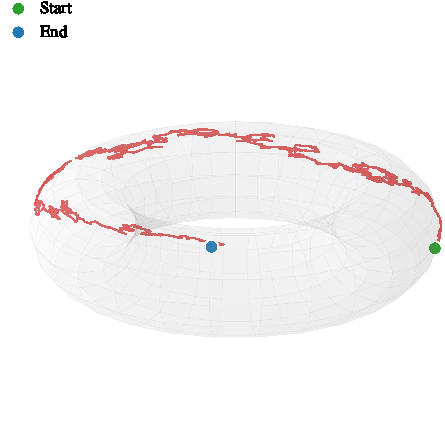
\includegraphics[width=0.30\textwidth]{fig_trajectory_compact.pdf}
\vspace{-6pt}
\caption{Stochastic trajectory on $\mathbb{T}^{2}$ embedded in $\mathbb{R}^{3}$, integrated by CF-EES(2,5) for 600 steps.}
\label{fig:torus_trajectory}
\vspace{-10pt}
\end{wrapfigure}

Each RNA nucleotide has seven backbone dihedral angles
$(\alpha, \beta, \gamma, \delta, \epsilon, \zeta, \chi)$ that naturally
live on the flat $d$-torus $\mathbb{T}^{d} = \mathrm{SO}(2)^{d}$, the
simplest non-trivial compact Lie group.
We train a neural SDE on $\mathbb{T}^{7}$ for one-step-ahead torsion-angle
forecasting: given a 20-residue context window, predict the next residue's
seven dihedrals.  A GRU encoder over $(\sin\theta, \cos\theta)$ angle features
and nucleotide identity (A/C/G/U one-hot) produces a conditioning vector; drift
and diffusion MLPs parameterise the SDE whose retraction is the componentwise
wrap modulo $2\pi$ (Figure~\ref{fig:torus_trajectory}).  Training minimises the
wrapped energy score~\citep{gneiting2007strictly}, a strictly proper scoring rule
on the torus.  We train on 67{,}000 non-canonical residue pairs
(those whose torsion vector lies $> 1\,\mathrm{rad}$ from the training circular mean)
drawn from 3{,}000 BGSU representative RNA chains at 3.0\,\AA{} resolution, and
evaluate with 16-sample MC averaging.

\begin{wrapfigure}{r}{0.42\textwidth}
\vspace{-14pt}
\centering
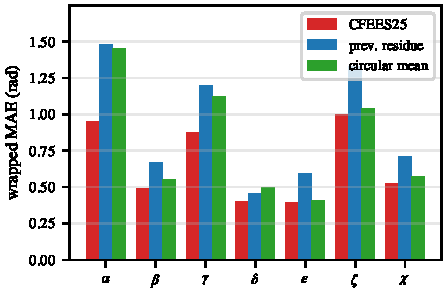
\includegraphics[width=0.40\textwidth]{fig_predictions_bar.pdf}
\vspace{-6pt}
\caption{Per-angle wrapped MAE on non-canonical test residues ($n = 17{,}682$).
CF-EES(2,5) (red) beats both the training circular mean (green) and the
predict-previous baseline (blue) on every angle.}
\label{fig:torus_bar}
\vspace{-10pt}
\end{wrapfigure}

On the non-canonical test set ($n = 17{,}682$), the model achieves an overall
wrapped MAE of $0.663\,\mathrm{rad}$ against $0.807\,\mathrm{rad}$ for the
training circular mean --- an $\mathbf{17.9\%}$ relative reduction --- and beats
the baseline on all seven angles (Figure~\ref{fig:torus_bar}).
The largest margins are on the two most multimodal backbone torsions:
$\alpha$ at $+34.6\%$ (gauche$^{+}$/trans split) and $\gamma$ at $+22.2\%$
(backbone crankshaft motion).

\begin{wrapfigure}{r}{0.42\textwidth}
\vspace{-14pt}
\centering
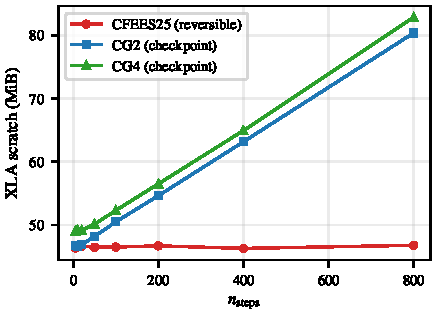
\includegraphics[width=0.40\textwidth]{fig_scaling_compact.pdf}
\vspace{-6pt}
\caption{XLA compile-time scratch for one forward+backward step at $d = 350$,
batch $32$.  CF-EES(2,5) under \texttt{ReversibleAdjoint} (red) is flat at
$46.5\,\mathrm{MiB}$; CG2/CG4 under checkpointing grow linearly.}
\label{fig:torus_scaling}
\vspace{-10pt}
\end{wrapfigure}

Because the torus is a flat abelian Lie group, this experiment cleanly isolates
the $\mathcal{O}(1)$ memory claim from the noncommutative geometry exercised by
the SPD companion.  At state dimension $d = 350$ and batch $32$,
$\mathrm{CF\text{-}EES}(2,5)$ under \texttt{ReversibleAdjoint} stays constant
at $46.5\,\mathrm{MiB}$ of XLA scratch across
$n_{\mathrm{steps}} \in [5, 800]$, while CG2 and CG4 under
one-snapshot-per-step checkpointing grow linearly at
$0.043\,\mathrm{MiB}$/step (Figure~\ref{fig:torus_scaling}).
The ratio reaches $1.72\times$ at $n_{\mathrm{steps}} = 800$ and extrapolates
to $10.2\times$ at $10{,}000$.  Full architecture and dataset details are in
Appendix~\ref{app:torus_details}.

\bibliography{neurips_references}
\bibliographystyle{plainnat}
\clearpage
\appendix
\section{Homogenous Space Integrators and Commutator-free \texorpdfstring{$\mathrm{EES}(2,5;x)$}{EES(2,5;x)}}

This section introduces geometric numerical integration over homogeneous spaces as an extension of the well-known Lie group case and describe the SPD geometry of our experiments. We then provide some background on commutator-free methods, of which our $\mathrm{CF-EES}(2,5;x)$ belongs, and show its memory-compute optimality.

\subsection{Symmetric Integration over Homogenous Spaces}
\label{subsec:homogenous_space_integration}
For chart-based Homogeneous space integrators, selfadjointness depends not only on the Butcher tableau of the underlying method, but also requires the chosen local coordinates are compatible with time reversal. There are two natural ways to enforce this:
\begin{enumerate}[label=(\roman*)]
  \item use symmetric coordinates, centered at a geodesic or flow midpoint, in the style of self-adjoint Lie-group methods \cite{Zanna2001},
  \item or use an embedded frozen-flow model whose frozen dynamics already integrate to an exactly
reversible map on \(M\).
\end{enumerate}

The first route is intrinsic, but generally leads to midpoint-centered constructions and hence away from the present
explicit frozen-flow framework. The second route is the one used here, which works for arbitrary homogeneous spaces.

Consider a homogeneous space $M$ endowed with a transitive action $\Lambda \colon G \times M \to M$
of a Lie group $G$. Rather than working with vector fields on $M$ directly, the key idea is to
represent them through elements of the Lie algebra $\mathfrak{g} = T_eG$: each $v \in \mathfrak{g}$
acts on $M$ via the \textbf{fundamental vector field}
\begin{equation}
    v_M(y) \coloneqq \frac{\mathrm{d}}{\mathrm{d}t}\bigg|_{t=0} \Lambda(\exp(tv),\, y),
\end{equation}
the infinitesimal version of the group action. A vector field $F$ on $M$ is then represented
through a state-dependent generator $\xi(y) \in \mathfrak{g}$ via $F(y) = \xi(y)_M(y)$,
replacing the role that Lie-algebra multiplication $vy$ plays on the group itself:
\begin{equation}
    gh \rightsquigarrow \Lambda(g,y), \qquad vy \rightsquigarrow v_M(y),
\end{equation}
for $g \in G$, $v \in \mathfrak{h}_y/\mathfrak{g}$, $y \in M$. This substitution lifts standard Lie-group
integration schemes from $G$ to $M$. In general, this construction is only unique up to the isotopy algebra $\mathfrak{h}_y = \{A \in \mathfrak{g} \colon A_m(y) = 0\}$, the set of generators whose induced vector field at $y$ is zero and thus produce no tangent motion. An example is given in Example~\ref{ex:isotropy}. To avoid this one fixes a representative of each tangent direction, typically by choosing a complement to the isotropy algebra and lifting only through that subspace.

\begin{road2}
\begin{example}[Example of degenerate choices due to the isotropy algebra]
\label{ex:isotropy}
Consider the sphere $S^2 \simeq \mathrm{SO}(3)/\mathrm{SO}(2)$ with the standard transitive action of $\mathrm{SO}(3)$ on $S^2 \subset \mathbb{R}^3$. At the north pole $p = e_3$, the isotropy subgroup is
\[
H_p = \{ R \in \mathrm{SO}(3) : Rp = p \} \simeq \mathrm{SO}(2),
\]
namely the rotations about the vertical axis. Its Lie algebra consists of the infinitesimal rotations that leave $p$ fixed to first order.

Equivalently, if $K \in \mathfrak{so}(3)$ generates a rotation about the $e_3$-axis, then its fundamental vector field vanishes at $p$:
\[
K_{S^2}(p)
=
\frac{\mathrm{d}}{\mathrm{d}t}\bigg|_{t=0} \exp(tK)p
=
0.
\]
Hence, if $A \in \mathfrak{so}(3)$ represents some tangent vector at $p$, then so does $A+K$ for any such $K$, since
\[
(A+K)_{S^2}(p) = A_{S^2}(p) + K_{S^2}(p) = A_{S^2}(p).
\]
Thus the lift of a tangent vector from $T_pS^2$ to $\mathfrak{so}(3)$ is not unique: one may add any element of the isotropy algebra without changing the induced tangent motion at $p$.
\end{example}
\end{road2}


The reverse of a frozen homogeneous-space flow is obtained by changing the sign of \(t\). Indeed, for a fixed generator \(v \in \mathfrak{g}\), by the group action identity \(\Lambda\) gives
\begin{equation}
    \Lambda\!\left(\exp(-tv), \Lambda(\exp(tv), y_0)\right)
    =
    \Lambda\!\left(\exp(-tv)\exp(tv), y_0\right)
    =
    \Lambda(e, y_0)
    =
    y_0.
\end{equation}
Hence the frozen flow is exactly reversible: its adjoint is obtained by time reversal, that is, by replacing \(t\) with \(-t\). This is a property of the frozen flow itself, before any recomputation of the generator along the trajectory.

\subsection{Construction of Self-adjoint SPD Geometry}
\label{subsec:spd_geometry}
We now make our construction concrete for the SPD experiment of Section~\ref{subsec:experiment_manifold_sde}.
The SPD manifold $\mathcal{S}_{++}^n \simeq \mathrm{GL}(n)/\mathrm{O}(n)$ carries the transitive
$\mathrm{GL}(n)$-action
\begin{equation}
    \Lambda(g, P) = g P g^\top,
\end{equation}
so the natural algebra for generating tangent directions is $\mathfrak{gl}(n)$. The network outputs
$x \in \mathbb{R}^{n(n+1)/2}$, which is mapped to a symmetric matrix
$A \in \mathrm{Sym}(n) \subseteq \mathfrak{gl}(n)$, a Lie-algebra element that acts on the current
state $P$ to produce a tangent vector. Applying the fundamental vector field construction gives
\begin{equation}
    A_{\mathcal{S}_{++}}(P)
    = \frac{\mathrm{d}}{\mathrm{d}t}\bigg|_{t=0} e^{tA} P e^{tA^\top}
    = AP + PA^\top,
\end{equation}
which, since $A^\top = A$, reduces to $AP + PA$. The vector field on $\mathcal{S}_{++}^n$ is
therefore $F(P) = AP + PA$, with $A \in \mathfrak{gl}(n)$ playing the role of $\xi(P)$. Freezing
this field and integrating exactly yields
\begin{equation}
    \dot{P} = AP + PA \implies P(t) = e^{tA} P_0 e^{tA},
\end{equation}
the Lie-group flow on $\mathcal{S}_{++}^n$ corresponding to the generator $A$.

The adjoint of this \emph{frozen} flow is obtained by reversing the sign of \(t\), giving
\begin{equation}
    P(-t) = e^{-tA} P e^{-tA^\top}.
\end{equation}
For fixed \(A\), this map is the exact inverse of the forward frozen flow. Indeed,
\begin{equation}
    e^{-tA} \bigl(e^{tA} P e^{tA^\top}\bigr) e^{-tA^\top}
    =
    \bigl(e^{-tA}e^{tA}\bigr)\, P \,\bigl(e^{tA^\top}e^{-tA^\top}\bigr)
    = IPI = P.
\end{equation}
Hence the frozen congruence flow on \(\mathcal{S}_{++}^n\) is self-adjoint, with a particularly simple exact inverse.

\subsection{Commutator-Free Integrators}
Commutator free (CF) \cite{celledoni_commutator-free_2003} generalize Crouch-Grossman (CG) \cite{crouch_numerical_1993} methods by allowing multiple exponentials per stage, while still avoiding the explicit evaluation of commutators as in Runge--Kutta Munthe--Kaas methods \cite{munthe-kaasRungeKuttaMethodsLie1998}.

For simplicity, we present the autonomous case; the non-autonomous case is handled by the standard augmentation in time. Given internal stage values $Y_i \in M$, we evaluate the left-trivialized stage slopes
\begin{equation}
    K_i = f(Y_i) \in \mathfrak{g}, \qquad i=1,\dots,s. \tag{left-trivialized slope}
\end{equation}
Each stage is then formed by acting on the current state $y_n$ with an ordered product of exponentials of linear combinations of previously computed slopes
\begin{equation}
    Y_i
    =
    \Lambda\!\left(
        \mathcal{T}\left\{
            \prod_{l=1}^{L_i}
            \exp\left(
                h \sum_{j=1}^{i-1} a_{l;ij}\,K_j
            \right)
        \right\},
        y_n
    \right),
    \qquad i=1,\dots,s. \tag{stage equation}
\end{equation} 
where $Y_i$ is the stage value and $y_{n+1}$ is the next solution point. The step update then takes the form,
\begin{equation}
    y_{n+1}
    =
    \Lambda\!\left(
        \mathcal{T}\left\{
            \prod_{l=1}^{L}
            \exp\left(
                h \sum_{i=1}^{s} \beta_{l;i}\,K_i
            \right)
        \right\},
        y_n
    \right), \tag{update equation}
\end{equation}
where $L_i$ and $L$ denote the numbers of exponentials used in stage $i$ and in the final update, respectively, and $\mathcal{T}$ denotes ordered multiplication in $G$, with smaller indices appearing to the right.

\subsection{Adjoint Sensitivities for Commutator-Free Neural ODEs}
The continuous adjoint system underlying $\mathrm{CFEES}$ is obtained by applying \citet[Theorem~4.5]{wotte_geometric_2025} through the homogeneous-space lift introduced in Section~\ref{subsec:homogenous_space_integration} and specialized in Section~\ref{subsec:spd_geometry}. In the SPD case, this requires no further construction beyond the fixed symmetric lift $A \in \mathrm{Sym}(n)$.

\subsection{Theoretical Compute and Memory Requirements of Lie Group Integrators}
\luke{standardise flops per eval, and per exp. Then with fixed per-eval flops, compare total cost due to number of exps and evals (decomposed), then same for memory}
The dominant cost of Lie group integrators is the evaluation of exponentials.
In an \(s\)-stage Crouch--Grossman (CG) method, stage \(i\) uses \(i-1\) exponentials and the final update uses \(s\) more, giving
\[
N_{\exp}^{\mathrm{CG}}(s)
=
\sum_{i=1}^s (i-1) + s
=
\frac{s(s+1)}{2}.
\]
Thus, the exponential count of CG grows quadratically with the number of stages.

A general commutator-free (CF) method instead exponentiates linear combinations of previously computed stage slopes. Writing \(L_i\) for the number of exponentials used in stage \(i\) and \(L\) for the number used in the final update, its total exponential count is
\[
N_{\exp}^{\mathrm{CF}}(s)
=
\sum_{i=1}^s L_i + L.
\]
CG is recovered as the special case \(L_i=i-1\) and \(L=s\). In practice, CF methods are designed so that \(L_i\) and \(L\) remain small, reducing the exponential count from quadratic to linear in \(s\). For example, the 3-stage and 4-stage commutator-free schemes of Celledoni, Marthinsen, and Owren require \(3\) and \(5\) exponentials per step, respectively.

A particularly efficient instance is the 2N-storage commutator-free form of Bazavov, which reuses exponentials across stages and requires exactly one exponential per stage. Its per-step exponential count is therefore
\[
N_{\exp}^{\mathrm{2N\text{-}CF}}(s)=s,
\]
while the storage remains fixed at two registers.

\begin{table}[h]
\centering
\caption{Per-step exponential counts for \(s\)-stage Lie group integrators. We denote the methods of \cite{celledoni_commutator-free_2003} CMO CF.}
\label{tab:exp_counts}
\begin{tabular}{lccc}
\toprule
Method & \(s=3\) & \(s=4\) & \(s=5\) \\
\midrule
CG & \(6\) & \(10\) & \(15\) \\
CMO CF3/CF4 & \(3\) & \(5\) & -- \\
2N-CF & \(3\) & \(4\) & \(5\) \\
\bottomrule
\end{tabular}
\end{table}

\section{Rooted Trees and B-Series for RDEs}
\luke{This section requires additions: Planarly branched rough paths, a brief description of manifold rough integration. or maybe we just hope no one asks? this could be a lot for an appendix. We may wish to place this before the diffgeo section above too}
\subsection{The Connes-Kreimer Hopf Algebra}
%%%%%%%%%%%%%%%%%%%%%%%%%%%%%%%%%%%%%%%%%%%%%%%%%%

We give a brief account of non-planar (labelled) rooted trees and the Connes-Kreimer Hopf algebra. We refer the reader to \cite{hoffman2003hopf} for a comprehensive presentation. A non-planar labelled rooted tree is defined as a graph $\tau = (V, E, r)$ with vertex set $V$, edge set $E$ and a root vertex $r \in V$, together with a set of vertex decorations drawn from $\{1, \ldots, d\}$. We denote the empty tree by $\emptyset$. Given trees $\tau_1, \ldots, \tau_m$, we write $[\tau_1, \ldots, \tau_m]_a$ to denote the tree formed by connecting the root vertices of $\tau_1, \ldots, \tau_m$ to a new root, which receives the label $a \in \{1, \ldots, d\}$. Non-planarity means that the order of the trees in $[\tau_1, \ldots, \tau_m]_a$ is irrelevant. Repeated trees will be denoted using power notation, for instance
\begin{equation*}
    [\tau_1,\tau_1, \tau_2, \tau_3, \tau_3, \tau_3]_a = [\tau_1^2, \tau_2, \tau_3^3]_a.
\end{equation*}

We write $|\tau|$ to denote the number of vertices in a tree. Additionally, we define the following combinatorial quantities, defined on unlabelled trees:
\begin{align*}
    \emptyset! &= 1, \quad \bullet! = 1, \quad [\tau_1, \ldots, \tau_m]! = |[\tau_1, \ldots, \tau_m]| \prod_{i=1}^m \tau_i!,\\
    \sigma(\emptyset) &= 1, \quad \sigma(\bullet) = 1, \quad \sigma([\tau_1^{k_1}, \ldots, \tau_m^{k_m}]) = \prod_{i=1}^m k_i! \sigma(\tau_i)^{k_i},\\
    \beta(\emptyset) &= 1, \quad \beta(\bullet) = 1, \quad \beta([\tau_1^{k_1}, \ldots, \tau_m^{k_m}]) = \binom{[\tau_1^{k_1}, \ldots, \tau_m^{k_m}]}{|\tau_1|, \ldots, |\tau_m|}\prod_{i=1}^m \frac{1}{k_i!} \beta(\tau_i)^{k_i}.
\end{align*}

We will refer to the commutative juxtaposition of trees as a forest. We write $\mathcal{T}$ to denote the set of all non-planar labelled rooted trees, and $\mathcal{T}_N \subset \mathcal{T}$ to denote the trees $\tau$ with $|\tau| \leq N$. The free commutative $\mathbb{R}$-algebra generated by $\mathcal{T}$ will be denoted $\mathcal{H}$. The Connes-Kreimer ~\citep{connes1999hopf} Hopf algebra on $\mathcal{H}$ is defined as follows. Multiplication $\mu : \mathcal{H} \otimes \mathcal{H} \to \mathcal{H}$ is defined as the commutative juxtaposition of two forests, extended linearly to $\mathcal{H}$. The multiplicative unit is defined to be the empty forest $\emptyset$. The counit map $\varepsilon: \mathcal{H} \to \mathbb{R}$ is defined by $\varepsilon(\emptyset) = 1$ and $\varepsilon(\tau) = 0$ for all non-empty trees $\tau \in \mathcal{H}$. The coproduct map is defined recursively by
\begin{align*}
    \Delta(\emptyset) &= \emptyset \otimes \emptyset,\\
    \Delta [\tau_1, \ldots, \tau_m]_a &= [\tau_1, \ldots, \tau_m]_a \otimes \emptyset + (\mathrm{id} \otimes B^a_+)(\Delta \tau_1 \cdots \Delta \tau_m),
\end{align*}
where $B^a_+(\tau_1 \cdots \tau_m) := [\tau_1 \cdots \tau_m]_a$ for a forest $\tau_1 \cdots \tau_m$. The definition is extended to a linear multiplicative map on $\mathcal{H}$. We will occasionally use Sweedler's notation
\begin{equation*}
    \Delta \tau = \sum_{(\tau)} \tau^{(1)} \otimes \tau^{(2)}
\end{equation*}
for the coproduct. We omit the definition of the antipode $S$ here, and instead refer the reader to ~\citep{manchon2004hopf, hoffman2003hopf}. We denote the dual of the Connes-Kreimer Hopf algebra by $\mathcal{H}^*$. For $\varphi_1, \varphi_2 \in \mathcal{H}^*$, the convolution product is defined by
\begin{equation*}
    \varphi_1 * \varphi_2 = \mu_\mathbb{R} \circ (\varphi_1 \otimes \varphi_2) \circ \Delta,
\end{equation*}
with $\mu_\mathbb{R} : \mathbb{R} \otimes \mathbb{R} \to \mathbb{R}$ denoting multiplication in $\mathbb{R}$.

%%%%%%%%%%%%%%%%%%%%%%%%%%%%%%%%%%%%%%%%%%%%%%%%%%
\subsection{B-Series Expansions of ODEs}\label{appendix:b_series_ode}
%%%%%%%%%%%%%%%%%%%%%%%%%%%%%%%%%%%%%%%%%%%%%%%%%%

For any tree $\tau \in \mathcal{T}$, the so-called elementary differential $F(\tau)(y)$ ~\citep{butcher2016numerical} is defined recursively by
\begin{align*}
    &F(\emptyset)(y) = y, \quad F(\bullet_i)(y) = f_i(y),\\
    &F([\tau_1, \tau_2, \ldots, \tau_m]_i)(y) = f^{(m)}_i(y)(F(\tau_1)(y), F(\tau_2)(y), \ldots, F(\tau_m)(y)).
\end{align*}

Given a map $\varphi: \mathcal{T} \to \mathbb{R}$, the associated B-series is defined
\begin{equation*}
    B_h(\varphi, y_0) := \sum_{\tau \in \mathcal{T}} \frac{h^{|\tau|}}{\sigma(\tau)} \varphi(\tau) F(\tau)(y_0).
\end{equation*}

A key property of B-series is their closure under composition. One can show that for two B-series \cite{hairer1974butcher, butcher2024b},
\begin{equation*}
    B_h(\varphi_2, B_h(\varphi_1, y_0)) = B_h(\varphi_1 * \varphi_2, y_0),
\end{equation*}
where $\varphi_1 * \varphi_2$ is the convolution product defined above. It can be shown that the exact solution to the ODE in \eqref{eq:ode} admits a B-series representation $y(h) = B_h(e, y_0)$, where $e(\tau) = 1 / \tau!$. Similarly, the solution given by a Runge--Kutta scheme with coefficients $\{a_{ij}\}_{1 \leq i,j \leq s}$, $\{b_i\}_{1 \leq i \leq s}$ admits the B-series representation $B_h(\varphi, y_0)$, where \cite[Lemma 312B]{butcher2016numerical}
\begin{equation*}
    \varphi(\tau) := \sum_{i_1, \ldots, i_n} b_{i_1} \prod_{(k,\ell) \in E} a_{i_k, i_\ell}
\end{equation*}
for a tree $\tau = (V,E,r)$ with $|\tau| = n$.\\

We refer the reader to ~\citep{hairer2006geometric,mclachlan2015butcher,butcher2021b} for a detailed account of B-series and the Butcher group.


%%%%%%%%%%%%%%%%%%%%%%%%%%%%%%%%%%%%%%%%%%%%%%%%%%
\subsection{Branched Rough Paths}\label{appendix:branched_rp}
%%%%%%%%%%%%%%%%%%%%%%%%%%%%%%%%%%%%%%%%%%%%%%%%%%

Let $\mathcal{H}$ be the Connes-Kreimer Hopf algebra of non-planar labelled rooted trees defined above.

\begin{definition}
    Let $\alpha \in (0,1]$. An $\alpha$-H\"older branched rough path is a map $\mathbf{X} : [0,T]^2 \to \mathcal{H}^*$ such that
    \begin{enumerate}
        \item for all $s,t \in [0,T]$ and $\tau_1, \tau_2 \in \mathcal{H}$,
        \begin{equation*}
            \langle \mathbf{X}_{s,t}, \tau_1 \rangle \langle \mathbf{X}_{s,t}, \tau_2 \rangle = \langle \mathbf{X}_{s,t}, \tau_1 \tau_2 \rangle,
        \end{equation*}
        \item for all $\tau \in \mathcal{H}$,
        \begin{equation*}
            \langle \mathbf{X}_{s,t}, \tau \rangle = \sum_{(\tau)} \langle \mathbf{X}_{s,u}, \tau^{(1)} \rangle \langle \mathbf{X}_{u, t}, \tau^{(2)} \rangle,
        \end{equation*}
        where $\Delta \tau = \sum_{(\tau)} \tau^{(1)} \otimes \tau^{(2)}$.
        \item for all $\tau \in \mathcal{H}$,
        \begin{equation*}
            \sup_{s \neq t} \frac{|\langle \mathbf{X}_{s,t}, \tau \rangle |}{|t - s| ^{\alpha |\tau|}} < \infty.
        \end{equation*}
    \end{enumerate}
\end{definition}

\begin{remark}
    As remarked in ~\citep{hairer2015geometric,gubinelli2010ramification}, the components $\langle \mathbf{X}_{s,t}, \tau \rangle$ with $|\tau| > N$ are determined by those with $|\tau| \leq N$, where $N$ is the largest integer such that $N \alpha \leq 1$.
\end{remark}

The space of $\alpha$-H\"older branched rough paths is a complete metric space under the metric

\begin{equation*}
    \varrho_\alpha(\mathbf{X}, \mathbf{Y}) := \sum_{\tau \in \mathcal{T}_N} \sup_{s \neq t} \frac{|\langle \mathbf{X}_{s,t} - \mathbf{Y}_{s,t}, \tau \rangle |}{|t - s|^{\alpha |\tau|}},
\end{equation*}

where $N = \lfloor 1 / \alpha \rfloor$.

\subsection{Manifold rough RK}

\begin{enumerate}
    \item Redmann-Riedel rough RK is valid for any euclidean RK scheme
    \item EES25 is a 2N RK scheme (normal tableau just with an extra constraint)
    \item EES25 is thus also a manifold scheme
    \item Redmann-Riedel still valid
\end{enumerate}

\section{Proofs and Additional Theorems}
\subsection{Proof of Theorem~\ref{thm:all-ees25-are-2n}: All $\mathrm{EES}(2,5;x)$ schemes are $2N$.}
\label{prf:all-ees25-are-2n}
\begin{proof}
Since $\mathrm{EES}(2,5;x)$ is a $3$-stage explicit Runge--Kutta method, it is enough to verify the relation given in Theorem~\ref{thm:2N_relationship}.. From the tableau of \ref{prop:EES_2_5},
\[
a_{21}=\frac{1+2x}{4(1-x)},\qquad
a_{31}=\frac{(4x-1)^2}{4(x-1)(1-4x^2)},\qquad
a_{32}=\frac{1-x}{1-4x^2},\qquad
b_1=x,\qquad b_2=\frac12.
\]
Direct substitution gives
\[
a_{32}(b_1-a_{21})
=
\frac{1-x}{1-4x^2}\left(x-\frac{1+2x}{4(1-x)}\right)
=
\frac{4x^2-2x+1}{4(2x-1)(2x+1)},
\]
and
\[
(a_{31}-a_{21})b_2
=
\frac12\left(
\frac{(4x-1)^2}{4(x-1)(1-4x^2)}
-
\frac{1+2x}{4(1-x)}
\right)
=
\frac{4x^2-2x+1}{4(2x-1)(2x+1)}.
\]
Thus \ref{thm:2N_relationship} holds identically in $x$, and $\mathrm{EES}(2,5;x)$ is Williamson $2N$ for every admissible $x$.
\end{proof}

\subsection{The Method \texorpdfstring{$\mathrm{EES}(2,7;\frac{1}{4}(2-\sqrt{2}))$}{EES(2,7)} is Also $2N$}
While the main text focuses on $\mathrm{EES}(2,5;x)$ methods, our approach extends naturally to $\mathrm{EES}(2,7;\tfrac{1}{4}(2-\sqrt{2}))$, which may better preserve gradient stability under especially long rollouts.

We first specialize \citet[Theorem.~2]{bazavov_2n-storage_2025} to the four-stage case with the following proposition.
\begin{theorem}[{\cite[Theorem~2]{bazavov_2n-storage_2025}}]
    For a $4$-stage explicit Runge--Kutta method, the Williamson $2N$ conditions are
    \begin{align}
    \label{eq:2n-4stage-1}
    a_{32}(b_1-a_{21})&=(a_{31}-a_{21})b_2,\\
    \label{eq:2n-4stage-2}
    a_{42}(b_1-a_{21})&=(a_{41}-a_{21})b_2,\\
    \label{eq:2n-4stage-3}
    a_{43}(b_2-a_{32})&=(a_{42}-a_{32})b_3.
    \end{align}
\end{theorem}

\begin{theorem}
    The method $\mathrm{EES}(2,7;\frac{1}{4}(2-\sqrt{2}))$ is a distinguished $2N$ scheme.
\end{theorem}

\begin{proof}
    \label{thm:ees27_is_2n}
    For $\mathrm{EES}\!\left(2,7;\tfrac14(2-\sqrt2)\right)$ one has
    \[
    a_{21}=\frac12(2-\sqrt2),\quad
    a_{31}=0,\quad
    a_{32}=\frac12\sqrt2,\quad
    a_{41}=\frac12(2-\sqrt2),\quad
    a_{42}=0,\quad
    a_{43}=\frac12\sqrt2,
    \]
    \[
    b_1=\frac14(2-\sqrt2),\qquad
    b_2=\frac14\sqrt2,\qquad
    b_3=\frac14\sqrt2.
    \]
    Then
    \[
    a_{32}(b_1-a_{21})
    =
    \frac12\sqrt2\left(\frac14(2-\sqrt2)-\frac12(2-\sqrt2)\right)
    =
    \frac14(1-\sqrt2),
    \]
    while
    \[
    (a_{31}-a_{21})b_2
    =
    \left(0-\frac12(2-\sqrt2)\right)\frac14\sqrt2
    =
    \frac14(1-\sqrt2),
    \]
    so \eqref{eq:2n-4stage-1} holds. Next,
    \[
    a_{42}(b_1-a_{21})=0=(a_{41}-a_{21})b_2,
    \]
    so \eqref{eq:2n-4stage-2} holds. Finally,
    \[
    a_{43}(b_2-a_{32})
    =
    \frac12\sqrt2\left(\frac14\sqrt2-\frac12\sqrt2\right)
    =
    -\frac14,
    \]
    and
    \[
    (a_{42}-a_{32})b_3
    =
    \left(0-\frac12\sqrt2\right)\frac14\sqrt2
    =
    -\frac14,
    \]
    so \eqref{eq:2n-4stage-3} holds. Therefore
    $\mathrm{EES}\!\left(2,7;\tfrac14(2-\sqrt2)\right)$ is also Williamson $2N$.
\end{proof}

\begin{remark}
    For a Williamson 2N scheme, the number of additional 2N constraints is $\frac{(s-1)(s-2)}{2}$. Thus, for a 2-stage explicit RK method, $\frac{(2-1)(2-2)}{2} = 0$, and the 2N scheme is trivial.
\end{remark}

\section{Additional Experiments}
\subsection{Stochastic Volatility}
We embed all stochastic volatility models in the RDE framework of \citet{bonesini_rough_2024}, which spans classical Black–Scholes \cite{Black1973} to contemporary rough volatility models \cite{gatheral_volatility_2014}.

\subsection{Molecular Dynamics}
Differentiable MD enables end-to-end force-field optimization by backpropagating through simulated trajectories, making it possible to fit against experimental observables, such as vibrational spectra, that reflect ensemble behaviour rather than static energy surfaces. The main challenge is that this requires differentiation through long Langevin trajectories, leading to memory costs linear in the rollout length and motivating specialized adjoints or checkpointing to remain tractable.

In this experiment, we fit an embedded neural network (EANN) 64-molecule water force field to experimental liquid-phase IR spectra, showing that $\mathrm{EES}(2,5)$ enables adjoint differentiation with $\mathcal{O}(1)$ memory in the rollout length for the full Langevin state $y_t = (r_t,v_t) \in \mathbb{R}^{6N_{\mathrm{atom}}} = \mathbb{R}^{1152}$. We adapt the deterministic setup of \textbf{cite} by replacing the velocity Verlet integrator with SDE solvers, while retaining the original dataset and training objective, now posed as a mean minimization problem.

We simulate finite-temperature Langevin trajectories and optimize the EANN parameters by matching the resulting infrared spectrum to experiment via the weighted squared loss over $B$ batches
\[
\mathcal{L}_{\mathrm{IR}}^{(B)}(\theta)
=
\frac{1}{B}
\sum_{b=1}^{B}
\left[
10 \sum_{\tilde{\nu} < 1000\,\mathrm{cm}^{-1}}
\left( I_{\theta}^{(b)}(\tilde{\nu}) - I^{\mathrm{exp}}(\tilde{\nu}) \right)^2
+
\sum_{1000 \leq \tilde{\nu} \leq 4000\,\mathrm{cm}^{-1}}
\left( I_{\theta}^{(b)}(\tilde{\nu}) - I^{\mathrm{exp}}(\tilde{\nu}) \right)^2
\right].
\]
Here \(I_{\theta}\) is computed from dipole autocorrelations along the simulated trajectory, so resolving the low-frequency bands requires differentiation through long stochastic rollouts of large state vectors.

We

Thus, EES integrators make tractable training even with extremely large state dimensions over long rollouts.

% \usepackage{tabularray}
% \UseTblrLibrary{booktabs}

\begin{table}[h]
\centering
\caption{Neural SDE training results across stochastic volatility models.}
\label{tab:atom_hparams}
\begin{tblr}{
  colspec = {llcccccc},
  row{1-2} = {font=\bfseries},
  rows = {abovesep=3pt, belowsep=3pt},
}
\toprule
Method & Problem & \SetCell[c=4]{c} W1 Loss & & & & Runtime (s) & Gradient error \\
       &         & 64 & 128 & 192 & 256 &             &                \\
\midrule
\SetCell[r=7]{c} {Reversible\\ Heun}
  & Black--Scholes          &       &       &       &       &       &       \\
  & Bergomi                 &       &       &       &       &       &       \\
  & Heston                  &       &       &       &       &       &       \\
  & Local                   &       &       &       &       &       &       \\
  & Rough Heston            &       &       &       &       &       &       \\
  & Quadratic rough Heston  &       &       &       &       &       &       \\
  & Rough Bergomi           &       &       &       &       &       &       \\
\bottomrule
\end{tblr}
\end{table}

\section{Experimental and Implementation Details}

\subsection{Additional Details for Torus SDE Experiments}
\label{app:torus_details}

\paragraph{Model.}
The state $\theta \in \mathbb{T}^{7}$ is integrated via the SDE
$\mathrm{d}\theta_\tau = f(\theta_\tau, c)\,\mathrm{d}\tau + g(\theta_\tau, c)\,\mathrm{d}W_\tau$,
initialised at the last observed angle $\theta_0 = \theta_t$.
The drift $f$ is a 4-layer MLP (width 384, ReLU) and the diffusion $g$ is a 3-layer MLP
(width 384, ReLU, final layer softplus at bias $-2.0$, scale $0.05$).
Both take $(\sin\theta, \cos\theta, c) \in \mathbb{R}^{14 + 64}$ as input, where
$c \in \mathbb{R}^{64}$ is the GRU encoder output.
The encoder processes per-step features $(\sin\theta, \cos\theta, \mathrm{onehot}(b))$
through a single-layer GRU (hidden 384).

\paragraph{Dataset.}
Representative RNA chains come from the BGSU non-redundant list at $3.0\,$\AA{} resolution,
parsed from mmCIF via \texttt{biotite}.
We retain contiguous runs of $\geq 30$ residues with all seven dihedrals defined.
Train/val/test splits are by chain-level deterministic hash (70/15/15\%).
We filter to \emph{non-canonical} targets: residues whose 7-dimensional torsion vector
lies $> 1\,\mathrm{rad}$ from the training circular mean (approximately 44\% of the data).
With \texttt{max\_chains}$= 3{,}000$ this yields 67{,}262 training and 17{,}682 test pairs.

\paragraph{Training.}
Wrapped energy score loss with $m = 4$ samples, AdamW at peak LR $10^{-4}$ with
cosine decay (5\% end), warmup 1{,}000 steps, gradient clipping at norm $1$, 20 epochs.
Test-time predictions are circular-meaned over 16 MC rollouts.

\paragraph{Memory scaling (Table~\ref{tab:torus_scaling}).}
\begin{table}[h]
\centering
\small
\caption{XLA compile-time scratch (MiB) for one forward+backward step at $d = 350$, batch $32$.}
\label{tab:torus_scaling}
\begin{tabular}{r rrr r}
\toprule
$n_{\mathrm{steps}}$ & CF-EES(2,5) & CG2 & CG4 & CG2/CF-EES \\
\midrule
  $5$   & $\mathbf{46.3}$ & $46.7$ & $49.0$ & $1.01\times$ \\
 $10$   & $\mathbf{46.5}$ & $46.5$ & $49.2$ & $1.00\times$ \\
 $20$   & $\mathbf{46.6}$ & $46.9$ & $49.2$ & $1.01\times$ \\
 $50$   & $\mathbf{46.5}$ & $48.2$ & $50.1$ & $1.04\times$ \\
$100$   & $\mathbf{46.5}$ & $50.5$ & $52.3$ & $1.09\times$ \\
$200$   & $\mathbf{46.7}$ & $54.6$ & $56.5$ & $1.17\times$ \\
$400$   & $\mathbf{46.3}$ & $63.2$ & $64.9$ & $1.37\times$ \\
$800$   & $\mathbf{46.8}$ & $80.4$ & $82.8$ & $1.72\times$ \\
\bottomrule
\end{tabular}
\end{table}

\paragraph{Per-angle forecasting accuracy (Table~\ref{tab:torus_mae}).}
\begin{table}[h]
\centering
\small
\caption{Per-angle wrapped MAE (rad) on 17{,}682 non-canonical test residues.}
\label{tab:torus_mae}
\begin{tabular}{l ccc c}
\toprule
Angle & CF-EES(2,5) & Circular mean & Prev.\ residue & Lift vs.\ mean \\
\midrule
$\alpha$   & $\mathbf{0.951}$ & $1.454$ & $1.481$ & $+34.6\%$ \\
$\beta$    & $\mathbf{0.491}$ & $0.551$ & $0.671$ & $+10.9\%$ \\
$\gamma$   & $\mathbf{0.874}$ & $1.123$ & $1.197$ & $+22.2\%$ \\
$\delta$   & $\mathbf{0.400}$ & $0.499$ & $0.456$ & $+19.8\%$ \\
$\epsilon$ & $\mathbf{0.394}$ & $0.405$ & $0.593$ & $+2.7\%$  \\
$\zeta$    & $\mathbf{1.000}$ & $1.043$ & $1.329$ & $+4.1\%$  \\
$\chi$     & $\mathbf{0.528}$ & $0.574$ & $0.712$ & $+8.0\%$  \\
\midrule
Overall    & $\mathbf{0.663}$ & $0.807$ & $0.920$ & $+17.9\%$ \\
\bottomrule
\end{tabular}
\end{table}

\subsection{Additional Details for SPD Manifold Experiments}
Daily closing prices for \texttt{AAPL}, \texttt{JPM}, \texttt{XOM}, \texttt{JNJ}, and \texttt{PG} are sourced from Yahoo Finance over the period 2005-01-01 to 2025-12-31, from which log-returns are computed. Rolling $5 \times 5$ empirical covariance matrices are then estimated using a 20-day window with Ledoit--Wolf shrinkage to improve conditioning \cite{Ledoit2004}. This results in 5 260 matrices, which are split 70/15/15\% across time.

\newpage
\input{checklist.tex}


\end{document}